
% NOTE!!!
%  Removing padding top from enumerate
% [noitemsep,topsep=0pt] (tambahkan setelah {}

  \subsection{Aliran Informasi}
  Subbab ini menjelaskan mengenai aliran data yang terjadi dalam proses-proses yang ada pada sistem. Rancangan aliran informasi secara umum dapat dilihat melalui diagram alur data level 0 pada gambar (..), dan secara lebih terperinci di alur data level 1 pada gambar (..)
      \begin{figure}[htp]
        \centering
        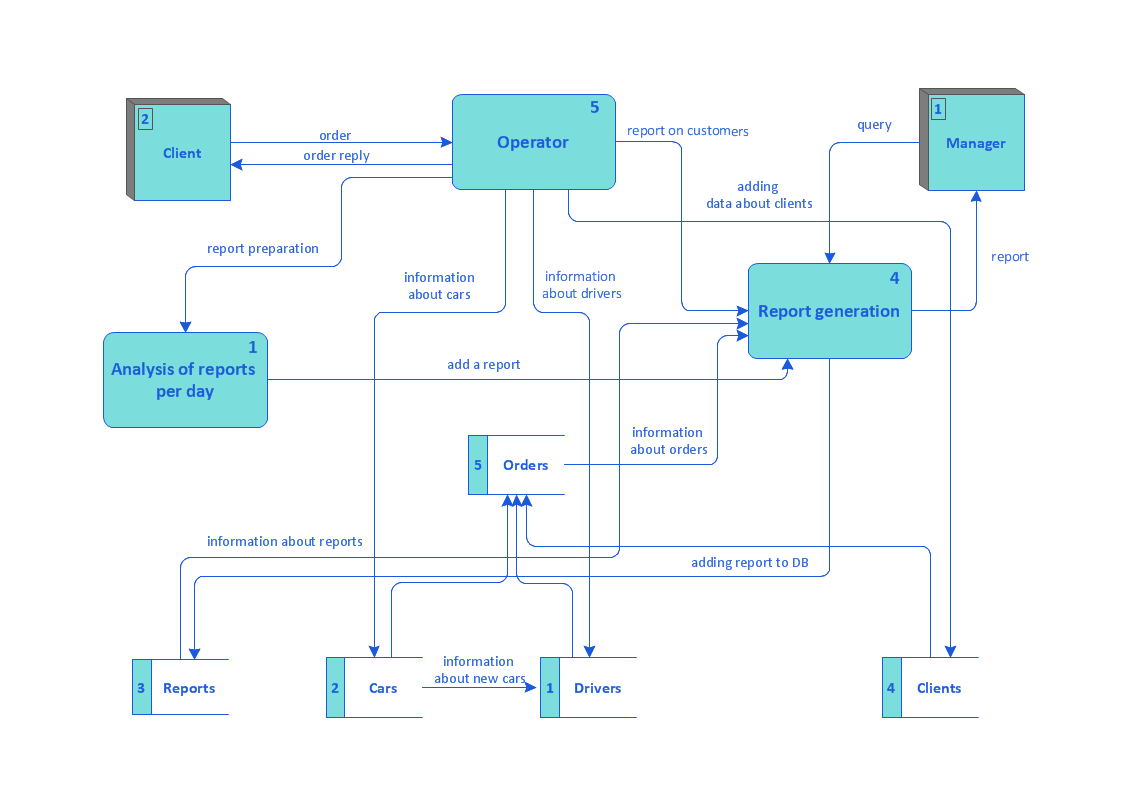
\includegraphics[width=1.0\columnwidth]{images/bab3/Taxi-service-dfd.png}
        \caption{DFD Level 0}
        \label{DFD0}
      \end{figure}
      
  \subsection{Deskripsi Proses}
  
  Pada subbab ini dijelaskan diagram alur data secara lebih mendetail pada proses-proses yang ada, yaitu proses I.
  
  \subsubsection{Proses I [Nama Proses]}
  Pengguna dapat ..... Detail Proses terdapat pada Gambar \ref{dfd1a} 
  
      \begin{figure}[htp]
        \centering
        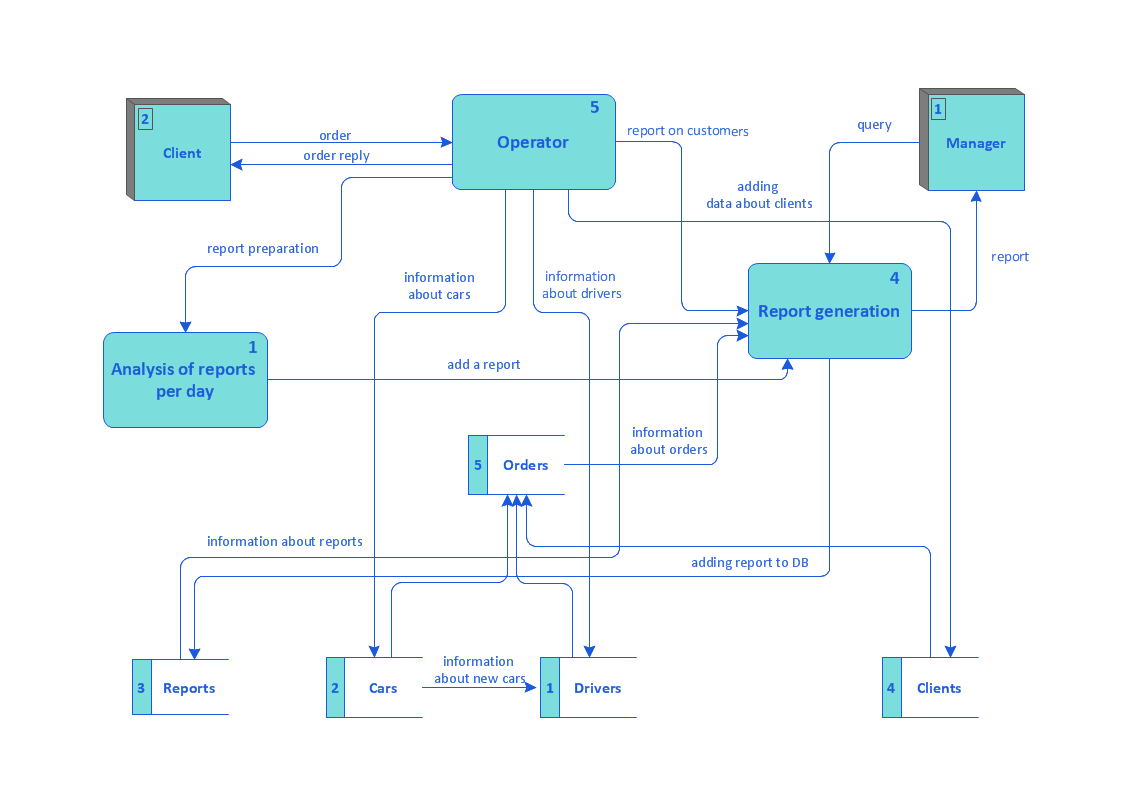
\includegraphics[width=\linewidth]{images/bab3/Taxi-service-dfd.png}
        \caption{DFD Level 1}
        \label{dfd1a}
      \end{figure}
      
  \subsubsection{Proses N [Nama Proses]}
  Pengguna dapat ..... Detail Proses terdapat pada Gambar \ref{dfd1n}
      \begin{figure}[H]
        \centering
        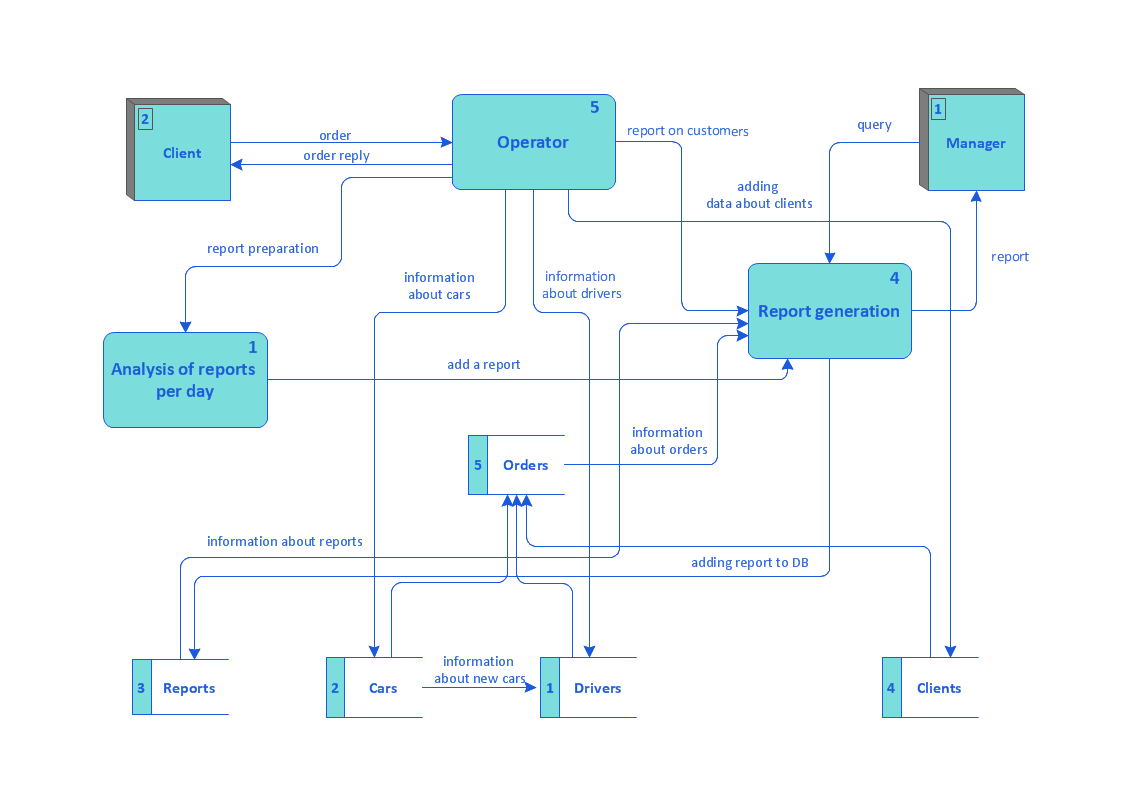
\includegraphics[width=\linewidth]{images/bab3/Taxi-service-dfd.png}
        \caption{DFD Level 1}
        \label{dfd1n}
      \end{figure}
  
  
  \subsection{Kamus Data}
  Pada bab ini dijelaskan kamus data dari entitas-entitas yang terlibat dalam sistem, sesuai dengan arus data yang telah dijelaskan.
 \subsubsection{Data Entitas 1}
 \indent Pada \textit{subsection} ini terdapat tabel berisi informasi entitas 1.
 \subsubsection{Data Entitas N}
 \indent Pada \textit{subsection} ini terdapat tabel berisi informasi entitas 1.
    
  \subsection{Pemodelan Data}
	\indent Pada subbab ini menjelaskan mengenai rancangan basis data sesuai dengan kebutuhan yang telah dijelaskan pada subbab sebelumnya. Basis Data dibangun menggunakan manajemen basis data PostgreSQL. \textit{Conceptual Data Model} (CDM) dipaparkan pada Gambar \ref{cdm}, dan \textit{Physical Data Model} dipaparkan pada Gambar \ref{pdm}.
      \begin{figure}[H]
        \centering
        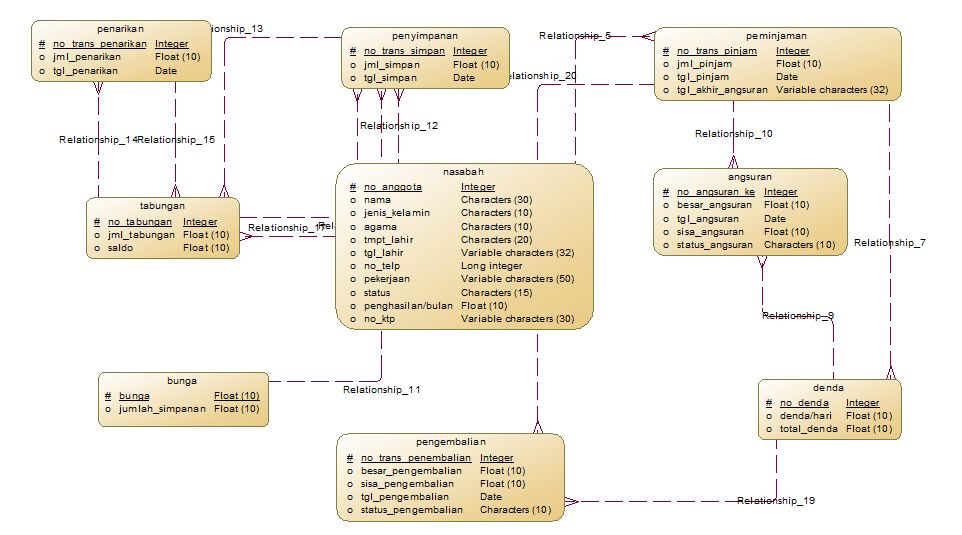
\includegraphics[width=\linewidth]{images/bab3/cdm.png}
        \caption{\textit{Conceptual Data Model} untuk aplikasi}
        \label{cdm}
      \end{figure}
      \begin{figure}[H]
        \centering
        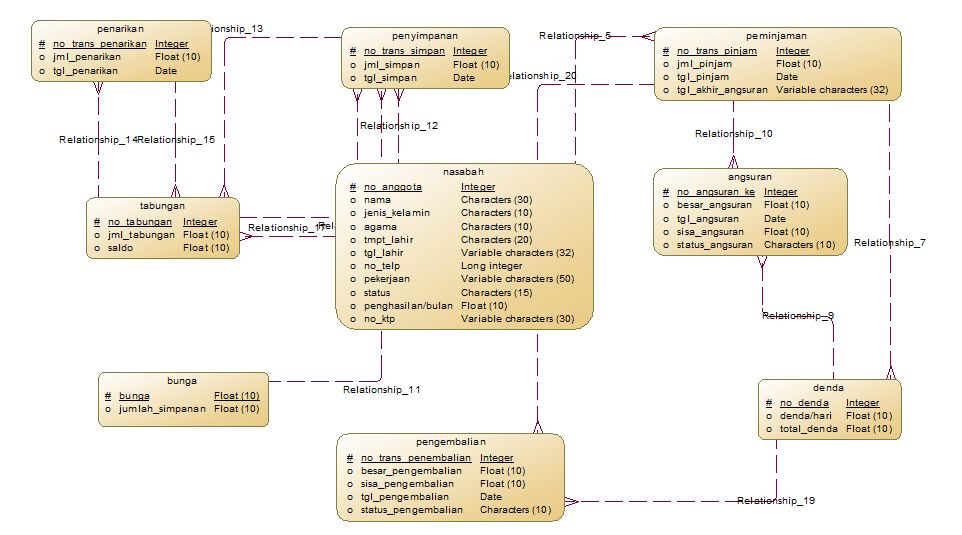
\includegraphics[width=\textwidth]{images/bab3/cdm.png}
        \caption{\textit{Physical Data Model} untuk aplikasi}
        \label{pdm}
      \end{figure}
      
  \subsection{Perancangan Arsitektur Sistem}
	Arsitektur sistem untuk aplikasi ini memiliki beberapa bagian utama, yaitu :
    \
\begin{enumerate}
\item \textit{web} server Nginx, berperan sebagai server
\item Database PostgreSQL, untuk penyimpanan data-data transaksional dan data lainnya selain 
\item Node.js untuk menyediakan data-data yang bersifat asinkronus seperti \textit{chatting} dan \textit{live bidding}.
\item MongoDB untuk penyimpanan data \textit{chat} dan riwayat \textit{chat} yang pernah dikirimkan pengguna
\end{enumerate}
	Untuk lebih jelasnya , dapat dilihat pada Gambar \ref{sysarch}
      \begin{figure}[H]
        \centering
        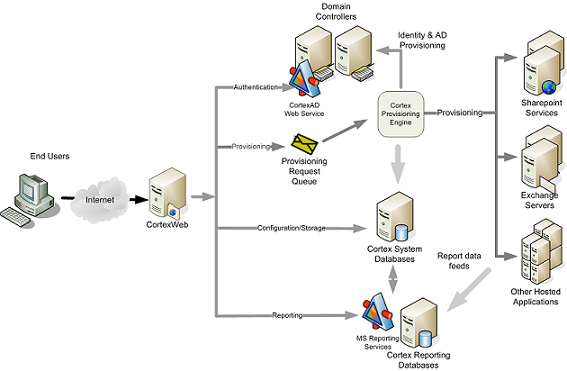
\includegraphics[width=\linewidth]{images/bab3/system-architecture.jpg}
        \caption{Arsitektur Sistem}
        \label{sysarch}
      \end{figure}